 \documentclass[a4paper,10pt]{article}

\usepackage{amsmath}
\usepackage{amstext}
\usepackage{amssymb}
\usepackage{amsfonts}
\usepackage{amsthm}
\usepackage{etoolbox}
%mathspec/fontspec
\usepackage{mathspec}
\usepackage{xunicode}
\usepackage{xltxtra}

\usepackage[bookmarks,bookmarksnumbered]{hyperref}

\makeatletter       % changes [1] to 1. in bibliography
\renewcommand{\@biblabel}[1]{#1.}
\makeatother

\usepackage{appendix}
\usepackage{graphicx}
\usepackage{natbib}


% FONT
\setmainfont[Mapping=tex-text,Numbers={Lining}]{Linux Libertine O}
\setmathfont(Latin)[Numbers={Lowercase}]{Linux Libertine O}
\setmathfont(Digits)[Scale=MatchLowercase]{Linux Libertine O}

\usepackage{unicode-math}
\setmainfont[Mapping=tex-text,Numbers={Lining}]{Linux Libertine O} 
\setmathfont{XITS Math}

\setmathfont[range={\mathup}]{Linux Libertine O} 
\setmathfont[range={\mathit}]{Linux Libertine O Italic} 
\setmathfont[range={\rm}]{Linux Libertine O} 
\setmathfont[range={\mathrm}]{Linux Libertine O} 



% \renewcommand{\rmdefault}{fxl}
\renewcommand{\sfdefault}{txss}


%%%%%%%%% from here yuasa setting %%%%%%%%%%%%%%%%%%%%%
% a4paper paperheight = 845.04684pt
%\setlength{\topmargin}{-.5in}
%% textheight = paperheight - 2in - \topmargin - \headheight - \headsep
%%              - \footskip = approx. 641pt
%\setlength{\textheight}{1.05\paperheight}
%\addtolength{\textheight}{-2.2in}
%%\addtolength{\textheight}{-\topmargin}
%%\addtolength{\textheight}{-\headheight}
%%\addtolength{\textheight}{-\headsep}
%%\addtolength{\textheight}{-\footskip}

%% a4paper paperwidth = 597.50787pt
%%\setlength{\marginparsep}{0pt}
%%\setlength{\marginparwidth}{0pt}
%% textwidth = paperwidth - 2in - \oddsidemargin = approx. 432pt
%\setlength{\textwidth}{\paperwidth}
%\addtolength{\textwidth}{-1.8in}
%%\addtolength{\textwidth}{-\oddsidemargin}

%% add 20pt to sidemargin
%%   oddside: 1in+20pt+20pt | \textwidth | 1in-20pt
%%   evenside: 1in-20pt | \textwidth | 1in+20pt+20pt
%\setlength{\oddsidemargin}{0pt}
%\setlength{\evensidemargin}{0pt}

%%%%%%%%% to here yuasa setting %%%%%%%%%%%%%%%%

%%%%%%%%% from here margin setting %%%%%%%%%%%%%%%%
%for dron
%\setlength{\topmargin}{0pt}
%\setlength{\marginparsep}{0pt}
%\setlength{\marginparwidth}{0pt}
%\setlength{\oddsidemargin}{20pt}
%\setlength{\evensidemargin}{0pt}
%
%\setlength{\textwidth}{\paperwidth}
%\addtolength{\textwidth}{-2in}
%\addtolength{\textwidth}{-\oddsidemargin}
%
%\addtolength{\oddsidemargin}{0pt}
%\addtolength{\evensidemargin}{-23pt}
%\setlength{\topmargin}{-12mm}
%\setlength{\textheight}{25.3cm}
%\setlength{\textwidth}{16.3cm}
%%%%%%%%% till here margin setting %%%%%%%%%%%%%%%%

%%% Linestrech
%for user guide
\renewcommand{\baselinestretch} {1.1}
%for dron
%\renewcommand{\baselinestretch} {1.1}

\setlength\bibsep{2pt}
\renewcommand{\bibnumfmt}[1]{(#1)}


%%% Table of Contents
\usepackage{tocloft}
\setlength\cftparskip{-0.7pt}
\setlength\cftbeforesecskip{1.5pt}
\setlength\cftaftertoctitleskip{2pt}

\addtolength{\oddsidemargin}{-.875in}
	\addtolength{\evensidemargin}{-.875in}
	\addtolength{\textwidth}{1.75in}

	\addtolength{\topmargin}{-.875in}
	\addtolength{\textheight}{1.75in}

%% for quotes
%\fontspec[Mapping=tex-text]{Linux Libertine O}
%\fontspec[Ligatures=TeX]{Linux Libertine O}

%%%%%%%%% color %%%%%%%%%
\usepackage{color}
\newcommand{\red}{\textcolor{red}}
\newcommand{\green}{\textcolor{green}}
\newcommand{\blue}{\textcolor[rgb]{0,0,0.8}}
\newcommand{\midnightblue}{\textcolor[rgb]{0.0976,0.0976,0.4375}}
\newcommand{\apricot}{\textcolor[rgb]{1,0,0.5}}
\newcommand{\strawberry}{\textcolor[rgb]{1,0,0.5}}
\newcommand{\orange}{\textcolor[rgb]{0.949, 0.593, 0}}
\newcommand{\gray}{\textcolor[rgb]{0.4,0.4,0.4}}
%%%%%%%%%%%%%%%%%%%%%%%%%%%


%%%%%%%%% for source code listing %%%%%%%%%
\usepackage{listings}


\lstset{%
 language={XML},
 backgroundcolor={\color[gray]{.97}},%
 basicstyle={\small\ttfamily},%
% identifierstyle={\small\ttfamily},%
 commentstyle={\gray},%
% keywordstyle={\small\bfseries\ttfamily},%
% ndkeywordstyle={\small},%
% stringstyle={\apricot},
 frame={tb},
 breaklines=true,
% columns=[l]{fullflexible},%
 numbers=left,%
% xrightmargin=5pt,%
% xleftmargin=5pt,%
% numberstyle={\scriptsize},%
% stepnumber=1,
 numbersep=5pt,%
 lineskip=-0.5pt,%
 showstringspaces=false,
 numbers=none
}
%%%%%%%%%%%%%%%%%%%%%%%%%%%

\title{\Huge{
SpaceWire RMAP GUI}\\
\Large{User Guide}}

\author{
{\Large
Takayuki Yuasa
}\\
{\small Japan Aerospace Exploration Agency, Institute of Space and Astronautical Science}\\
{\small yuasa \_at\_mark\_ astro.isas.jaxa.jp}\\
}

\date{January 11, 2012}

%\newcommand{\red}{\textcolor{red}}
%\newcommand{\green}{\textcolor{green}}
%\newcommand{\blue}{\textcolor{blue}}
%\newcommand{\apricot}{\textcolor[rgb]{1,0,0.5}}

\usepackage{listings}
\usepackage{color}

\lstset{%
 language={XML},
 backgroundcolor={\color[gray]{.97}},%
 basicstyle={\small\ttfamily},%
 identifierstyle={\small\ttfamily},%
 commentstyle={\small\ttfamily\itshape},%
 keywordstyle={\small\bfseries\ttfamily},%
 ndkeywordstyle={\small},%
 stringstyle={\small\ttfamily\apricot},
 frame={tb},
 breaklines=true,
% columns=[l]{fullflexible},%
 numbers=left,%
 xrightmargin=5pt,%
 xleftmargin=5pt,%
% numberstyle={\scriptsize},%
% stepnumber=1,
 numbersep=5pt,%
 lineskip=-0.5pt%
}

\begin{document}
\maketitle
\tableofcontents

\setcounter{page}{1}

%%%%%%%%%%%%%%%%%%%%%%%%%%%%%%%%%%%%%%
%%%%%%%%%%%%%%%%%%%%%%%%%%%%%%%%%%%%%%
\section{Overview}
\subsection{SpaceWire-to-GigabitEther}
SpaceWire-to-GigabitEther is an interface to SpaceWire networks for PC software via GigabitEthernet. Users can send/receive SpaceWire packets from/to a user program running on an ordinary PC to/from a SpaceWire node or router connected to the device. The class library written in C++ is also available for user programs which run on the PC. Using the library, users can perform Remote Memory Access Protocol (RMAP) to RMAP Target nodes connected to the converter through the SpaceWire network. This device is not flight qualified, but originally intended for SpaceWire/RMAP-based data acquisition system of scientific experiments and ground tests of flight modules which use SpaceWire interfaces.

Note that there are two types of SpaceWire-to-GigabitEther, one is an open-source version (FPGA IP and software are open), and the other is a product version which can be purchased from Shimafuji Electric.

\begin{itemize}
\item Open-source SpaceWire-to-GigabitEther utilizes the ZestET1 board by OrangeTree. SpaceWire Open IP (by Shimafuji Electric and Osaka University) and Host I/F are implemented on the UserFPGA of the board. This board bridges one TCP/IP connection to one external SpaceWire port.
\item Shimafuji's SpaceWire-to-GigabitEther provides very similar functionality as what the open-source version implements, but with an additional internal SpaceWire router and 4 micro-Dsub (MDM) external SpaceWire ports. The Shimafuji SpaceWire-to-GigabitEther accepts higher Tx frequencies (up to 200MHz) than the open-source version does (~130MHz).
\end{itemize}

The both SpaceWire-to-GigabitEther operates as a TCP server which listens/accepts a connection from a client PC on which user program runs. When disconnected, the converter goes back to the listening state and waits for a new connection. The Shimafuji SpaceWire-to-GigabitEther accepts two TCP/IP connections (identified by TCP/IP port numbers) and bridges them to separate SpaceWire ports (both connected to the internal SpaceWire router; see User Guide for details), while one TCP/IP-SpaceWire bridge is available in the open-source SpaceWire-to-GigabitEther.
Takayuki Yuasa currently concentrates on test/developments on the Shimafuji�fs SpaceWire-to-GigabitEther, and no big update for the open-source version will be expected due to limited man power.

\begin{figure}[htb]
\begin{center}
\begin{minipage}{0.45\hsize}
\begin{center}
\includegraphics[width=8cm]{figures/SpaceWire-to-GigabitEther/SpaceWire-to-GigabitEther_opensource_version.jpg}
\caption{Open-source SpaceWire-to-GigabitEther.}
\label{figure:openSourceSpWGbE}
\end{center}
\end{minipage}
\hspace{0.05\hsize}
\begin{minipage}{0.45\hsize}
\begin{center}
\includegraphics[width=8cm]{figures/SpaceWire-to-GigabitEther/SpaceWire-to-GigabitEther-Shimafuji-MDM4version.jpg}
\caption{Shimafuji Electric's SpaceWire-to-GigabitEther with 4 MDM SpaceWire ports.}
\label{figure:shimafujiSpWGbE}
\end{center}
\end{minipage}
\end{center}
\end{figure}


\subsection{SpaceWire RMAP GUI}
The GUI software SpaceWire RMAP GUI is available from the open-source SpaceWire project\footnote{The open-source SpaceWire project: \url{https://galaxy.astro.isas.jaxa.jp/~yuasa/SpaceWire}\label{url:supportpage}} on Mac.
Users can send/receive SpaceWire packets, and perform RMAP read/write transactions for debugging SpaceWire/RMAP devices.

\begin{figure}[htb]
\begin{center}
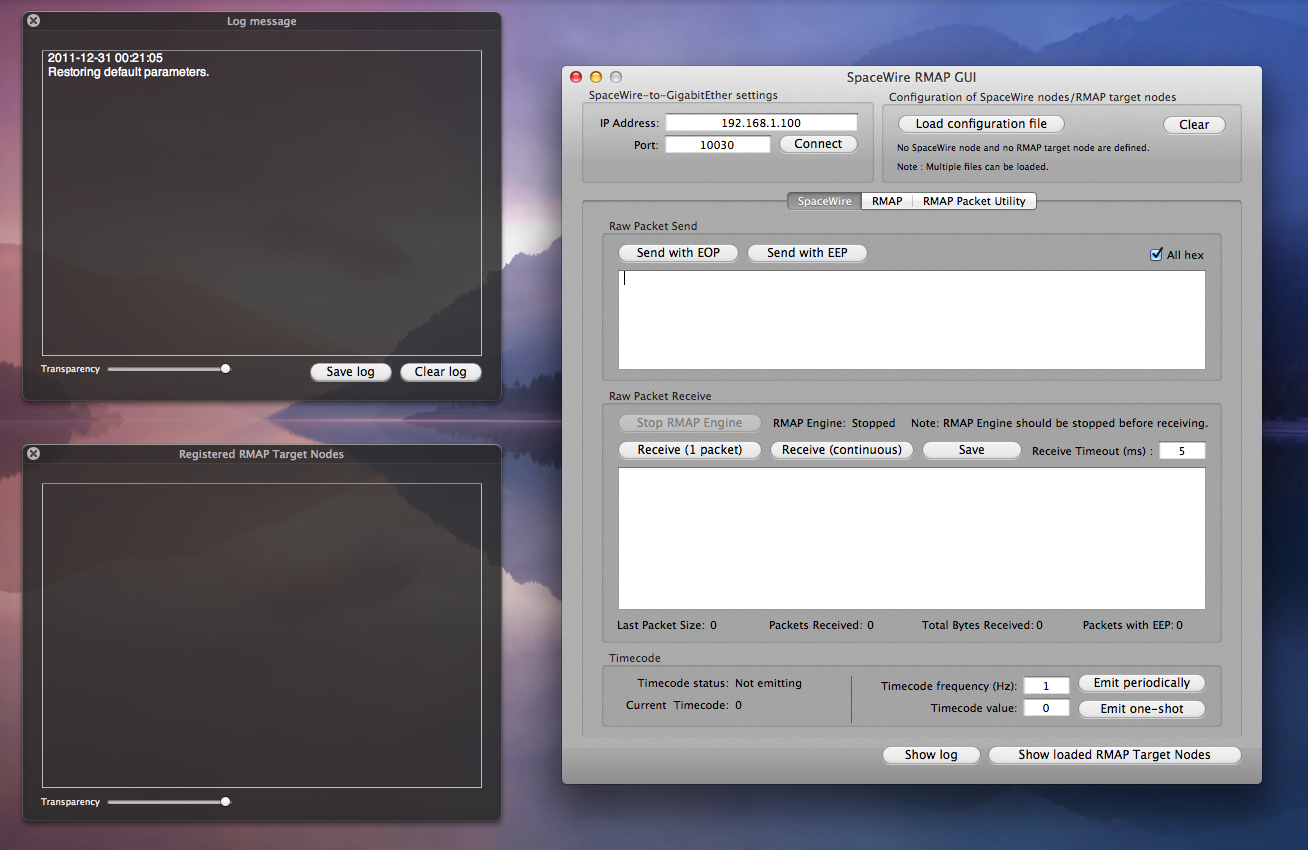
\includegraphics[width=12cm]{figures/SpaceWireRMAPGUI/Screenshot_all.png}
\caption{Screenshot of SpaceWire RMAP GUI.}
\label{figure:SpaceWireRMAPGUI}
\end{center}
\end{figure}


\subsection{This is an open-source user guide}

\subsection{Feedback}
\subsection{Revision}

\section{SpaceWire-to-GigabitEther}
\subsection{Purpose}
\subsection{Standalone version and AMC version}
\subsection{Specification}
\subsection{Dimensions}
\subsection{Weight}
\subsection{Power}

\subsection{Hardware block diagram}
\subsection{FPGA block diagram}
\subsection{Hardware implementation of a TCP/IP stack}
\subsection{Configuration of the internal SpaceWire router}
\subsection{Physical and internal SpaceWire connections}

\section{The internal SpaceWire Router}
\subsection{Basic design}
\subsection{Configurable items}
\subsection{Default parameters}
\subsection{Typical usages}
\subsection{Router Configuration Port (Port0)}
\subsection{Register Port (Port??)}
\subsection{Internal loop connection}

\section{Performance}
\subsection{SpaceWire packet transfer}
\subsection{RMAP data transfer}
\subsection{Performance of the VHDL TCP/IP stack}

\section{SpaceWire RMAP GUI}
\subsection{Overview}
This software is an open-source project.
No warranty, and provided as is.
\subsection{SpaceWire I/F control section}
\subsection{SpaceWire-layer operation}
\subsection{RMAP-layer operation}
\subsection{Define RMAP target nodes using an XML file}
\subsection{Define registers on RMAP target nodes using an XML file}
\subsection{RMAP Packet Utility}
\subsection{Scripting}

\section{Tutorial}
\subsection{Send/receive SpaceWire packets}
\subsection{Read/write access to an RMAP target node}
\subsection{Access the configuration port of the internal SpaceWire router}
\subsection{Access the routing table}
\subsection{Change link operating frequencies of SpaceWire ports}

\appendix
\chapter{TCP/IP-SpaceWire packet transfer protocol}
\chapter{Onboard CPU for configuration}
SpaceWire-to-GigabitEther implements a V850 processor for configuration via TCP/IP. 
\chapter{The SpaceWire/RMAP Library}

\end{document}